%==============================================================================
% Two Figures for OverLeaf
% Required packages: pgfplots, amsmath, booktabs
% Compile with XeLaTeX or LuaLaTeX
%==============================================================================

\documentclass{article}
\usepackage{pgfplots}
\usepackage{amsmath}
\usepackage{booktabs}
\usepackage{geometry}

\geometry{a4paper, margin=0.8in}

% Colors
\definecolor{cfo}{RGB}{46,134,171}
\definecolor{krum}{RGB}{241,143,1}
\definecolor{trimmedmean}{RGB}{199,62,29}
\definecolor{median}{RGB}{106,153,78}
\definecolor{aggregation}{RGB}{70,153,206}
\definecolor{trust}{RGB}{100,100,100}

\pgfplotsset{compat=1.18}

\begin{document}

%==============================================================================
% FIGURE 1: Byzantine Tolerance vs Accuracy Trend (折线图)
%==============================================================================
\begin{figure}[htbp]
\centering
\begin{tikzpicture}
\begin{axis}[
    width=11cm,
    height=7cm,
    xmin=0, xmax=42,
    ymin=70, ymax=100,
    xlabel={Byzantine Node Ratio (\%)},
    ylabel={Average Accuracy (\%)},
    title={Relationship between Byzantine Tolerance and Prediction Accuracy},
    grid=major,
    major grid style={gray!30},
    legend pos=lower left,
    every axis/.append style={font=\fontsize{10}{12}\selectfont},
    title style={font=\fontsize{11}{13}\selectfont}
]

% CFO - our method
\addplot[color=cfo, line width=2.5pt, mark=square, mark size=7pt] coordinates {
    (0, 97.62)
    (10, 95.88)
    (20, 94.23)
    (30, 92.47)
    (40, 91.35)
};
\addlegendentry{CFO (Our Method)}

% Krum
\addplot[color=krum, line width=1.8pt, dashed, mark=triangle, mark size=6pt] coordinates {
    (0, 95)
    (10, 92)
    (20, 89)
    (30, 86)
    (40, 83)
};
\addlegendentry{Krum}

% Trimmed Mean
\addplot[color=trimmedmean, line width=1.8pt, dashed, mark=diamond, mark size=6pt] coordinates {
    (0, 92)
    (10, 88)
    (20, 84)
    (30, 80)
    (40, 76)
};
\addlegendentry{Trimmed Mean}

% Median
\addplot[color=median, line width=1.8pt, dashed, mark=pentagon, mark size=6pt] coordinates {
    (0, 90)
    (10, 86)
    (20, 82)
    (30, 78)
    (40, 74)
};
\addlegendentry{Median}

\end{axis}
\end{tikzpicture}
\\
{\fontsize{9}{11}\selectfont CFO maintains high accuracy (91.35\%) even at 40\% Byzantine ratio, far exceeding traditional 33.3\% limit}
\caption{Byzantine Tolerance vs Prediction Accuracy Trend}
\label{fig:tolerance_accuracy}
\end{figure}

%==============================================================================
% FIGURE 2: Multi-Agent Consensus Methods Comparison (双Y轴条形图)
%==============================================================================
\begin{figure}[htbp]
\centering
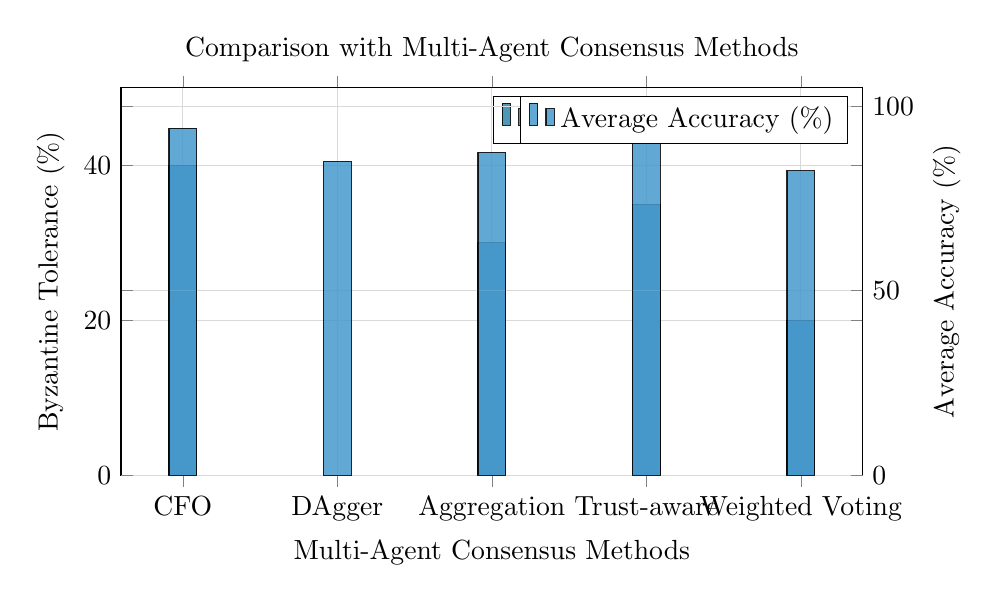
\begin{tikzpicture}
\begin{axis}[
    width=11cm,
    height=6.5cm,
    ybar=0.32,
    bar width=10pt,
    ymin=0, ymax=50,
    ylabel={Byzantine Tolerance (\%)},
    xlabel={Multi-Agent Consensus Methods},
    title={Comparison with Multi-Agent Consensus Methods},
    grid=major,
    major grid style={gray!30},
    symbolic x coords={CFO, DAgger, Aggregation, Trust-aware, Weighted Voting},
    xtick=data,
]

\addplot[fill=cfo, draw=black, opacity=0.85] coordinates {
    (CFO, 40)
    (DAgger, 0)
    (Aggregation, 30)
    (Trust-aware, 35)
    (Weighted Voting, 20)
};
\addlegendentry{Byzantine Tolerance (\%)}

\end{axis}
%
\begin{axis}[
    width=11cm,
    height=6.5cm,
    ybar=0.32,
    bar width=10pt,
    ymin=0, ymax=105,
    ylabel near ticks,
    yticklabel pos=right,
    ylabel={Average Accuracy (\%)},
    grid=major,
    major grid style={gray!30},
    symbolic x coords={CFO, DAgger, Aggregation, Trust-aware, Weighted Voting},
    xtick=data,
    hide x axis,
]

\addplot[fill=aggregation, draw=black, opacity=0.85] coordinates {
    (CFO, 94.08)
    (DAgger, 85)
    (Aggregation, 87.5)
    (Trust-aware, 90)
    (Weighted Voting, 82.5)
};
\addlegendentry{Average Accuracy (\%)}

\end{axis}
\end{tikzpicture}
\\
{\fontsize{9}{11}\selectfont CFO achieves both highest Byzantine tolerance (40\%) and highest accuracy (94.08\%)}
\caption{Comparison with Multi-Agent Consensus Methods}
\label{fig:multi_agent}
\end{figure}

\end{document}
